\chapter{Data Analysis}
\paragraph{}The goal for the MARATHON experiment is to determine the EMC effect for the two A=3 systems $^3$He and $^3$H, extract the  $F_2^n$/$F_2^p$, and calculate the $d$/$u$ quark distribution ratios. The goal of this analysis is to determine the EMC effect for the two A=3 systems via the ratio of measured cross sections. The cross-section of a scattering interaction is the probability of that event happening. In order to measure the probability of an event happening, a ratio has to be calculated between the magnitude of the number of those events versus the number of times that event could of happened. This analysis will use data from the HRSs, beam line detectors, and target information to measure the cross-section of $^3$He and $^3$H for kinematics of 0.2 $< x <$ 0.82. 
\section{Analysis Software}
\paragraph{}Hall A at JLab uses an analysis software (Analyzer) that is built on top of ROOT. The Analyzer is used to decode raw data received from TDCs, ADCs, and scalars into meaningful results. The decoding process uses raw data from the detectors in the HRSs and on the beam line to create an event. This event is assigned a track if applicable, and the events signal from the detectors are stored into a ROOT file. This ROOT file contains the raw and calibrated detector data from each signal, the track information, and physics variables calculated via the calibrated data and track information. 
\subsection{Tracking}
\paragraph{}The Analyzer uses calibrated VDC data to calculate the track of an event. The detector calibration was discussed in chapter \ref{ch:ExpUp}. The event tracking is used to determine the scattered angle and momentum of the electrons detected. The track determined from the VDCs is in reference to the detector coordinate system. The Analyzer uses a optics matrix to relate the tracking information between all coordinate systems used in the Hall A analysis process. The coordinate systems will be briefly discussed in this section. A more complete guide with in-depth discussion of the coordinate systems is discussed in \cite{espace}.
\begin{itemize}
	\item \textbf{Hall Coordinate System(HCS):} The intersection of the electron beam and the vertical symmetry axis of the target system defines the origin of the HCS. This allows for $\hat{z}$ to point along the beam line towards the beam dump and $\hat{y}$ is up. 
	\item \textbf{Target Coordinate System (TCS):} The TCS is unique to the individual HRS. The $\hat{z}$ axis of the TCS is defined by a line perpendicular to the surface of the spectrometers sieve slit aligned with the midpoint of the center hole. $z_{tg}$ points away from the target towards the spectrometer. Nilange Liyange states in reference \cite{optics}, "In the ideal case where the spectrometer is pointing directly at the hall center and the sieve slit is perfectly centered on the spectrometer, the z$_{tg}$ axis passes through the hall center." Using the idea case, the origin of the TCS is defined by a set distance from the sieve surface. For the Left HRS, the TCS origin is 1.181m from the sieve, and for the Right HRS it is 1.178m. In the ideal case, the TCS origin is the HCS origin. Figure \ref{fig:TCS} shows the TCS with a an electron scattering event from a foil. 
	\begin{figure}[]
		\centering
		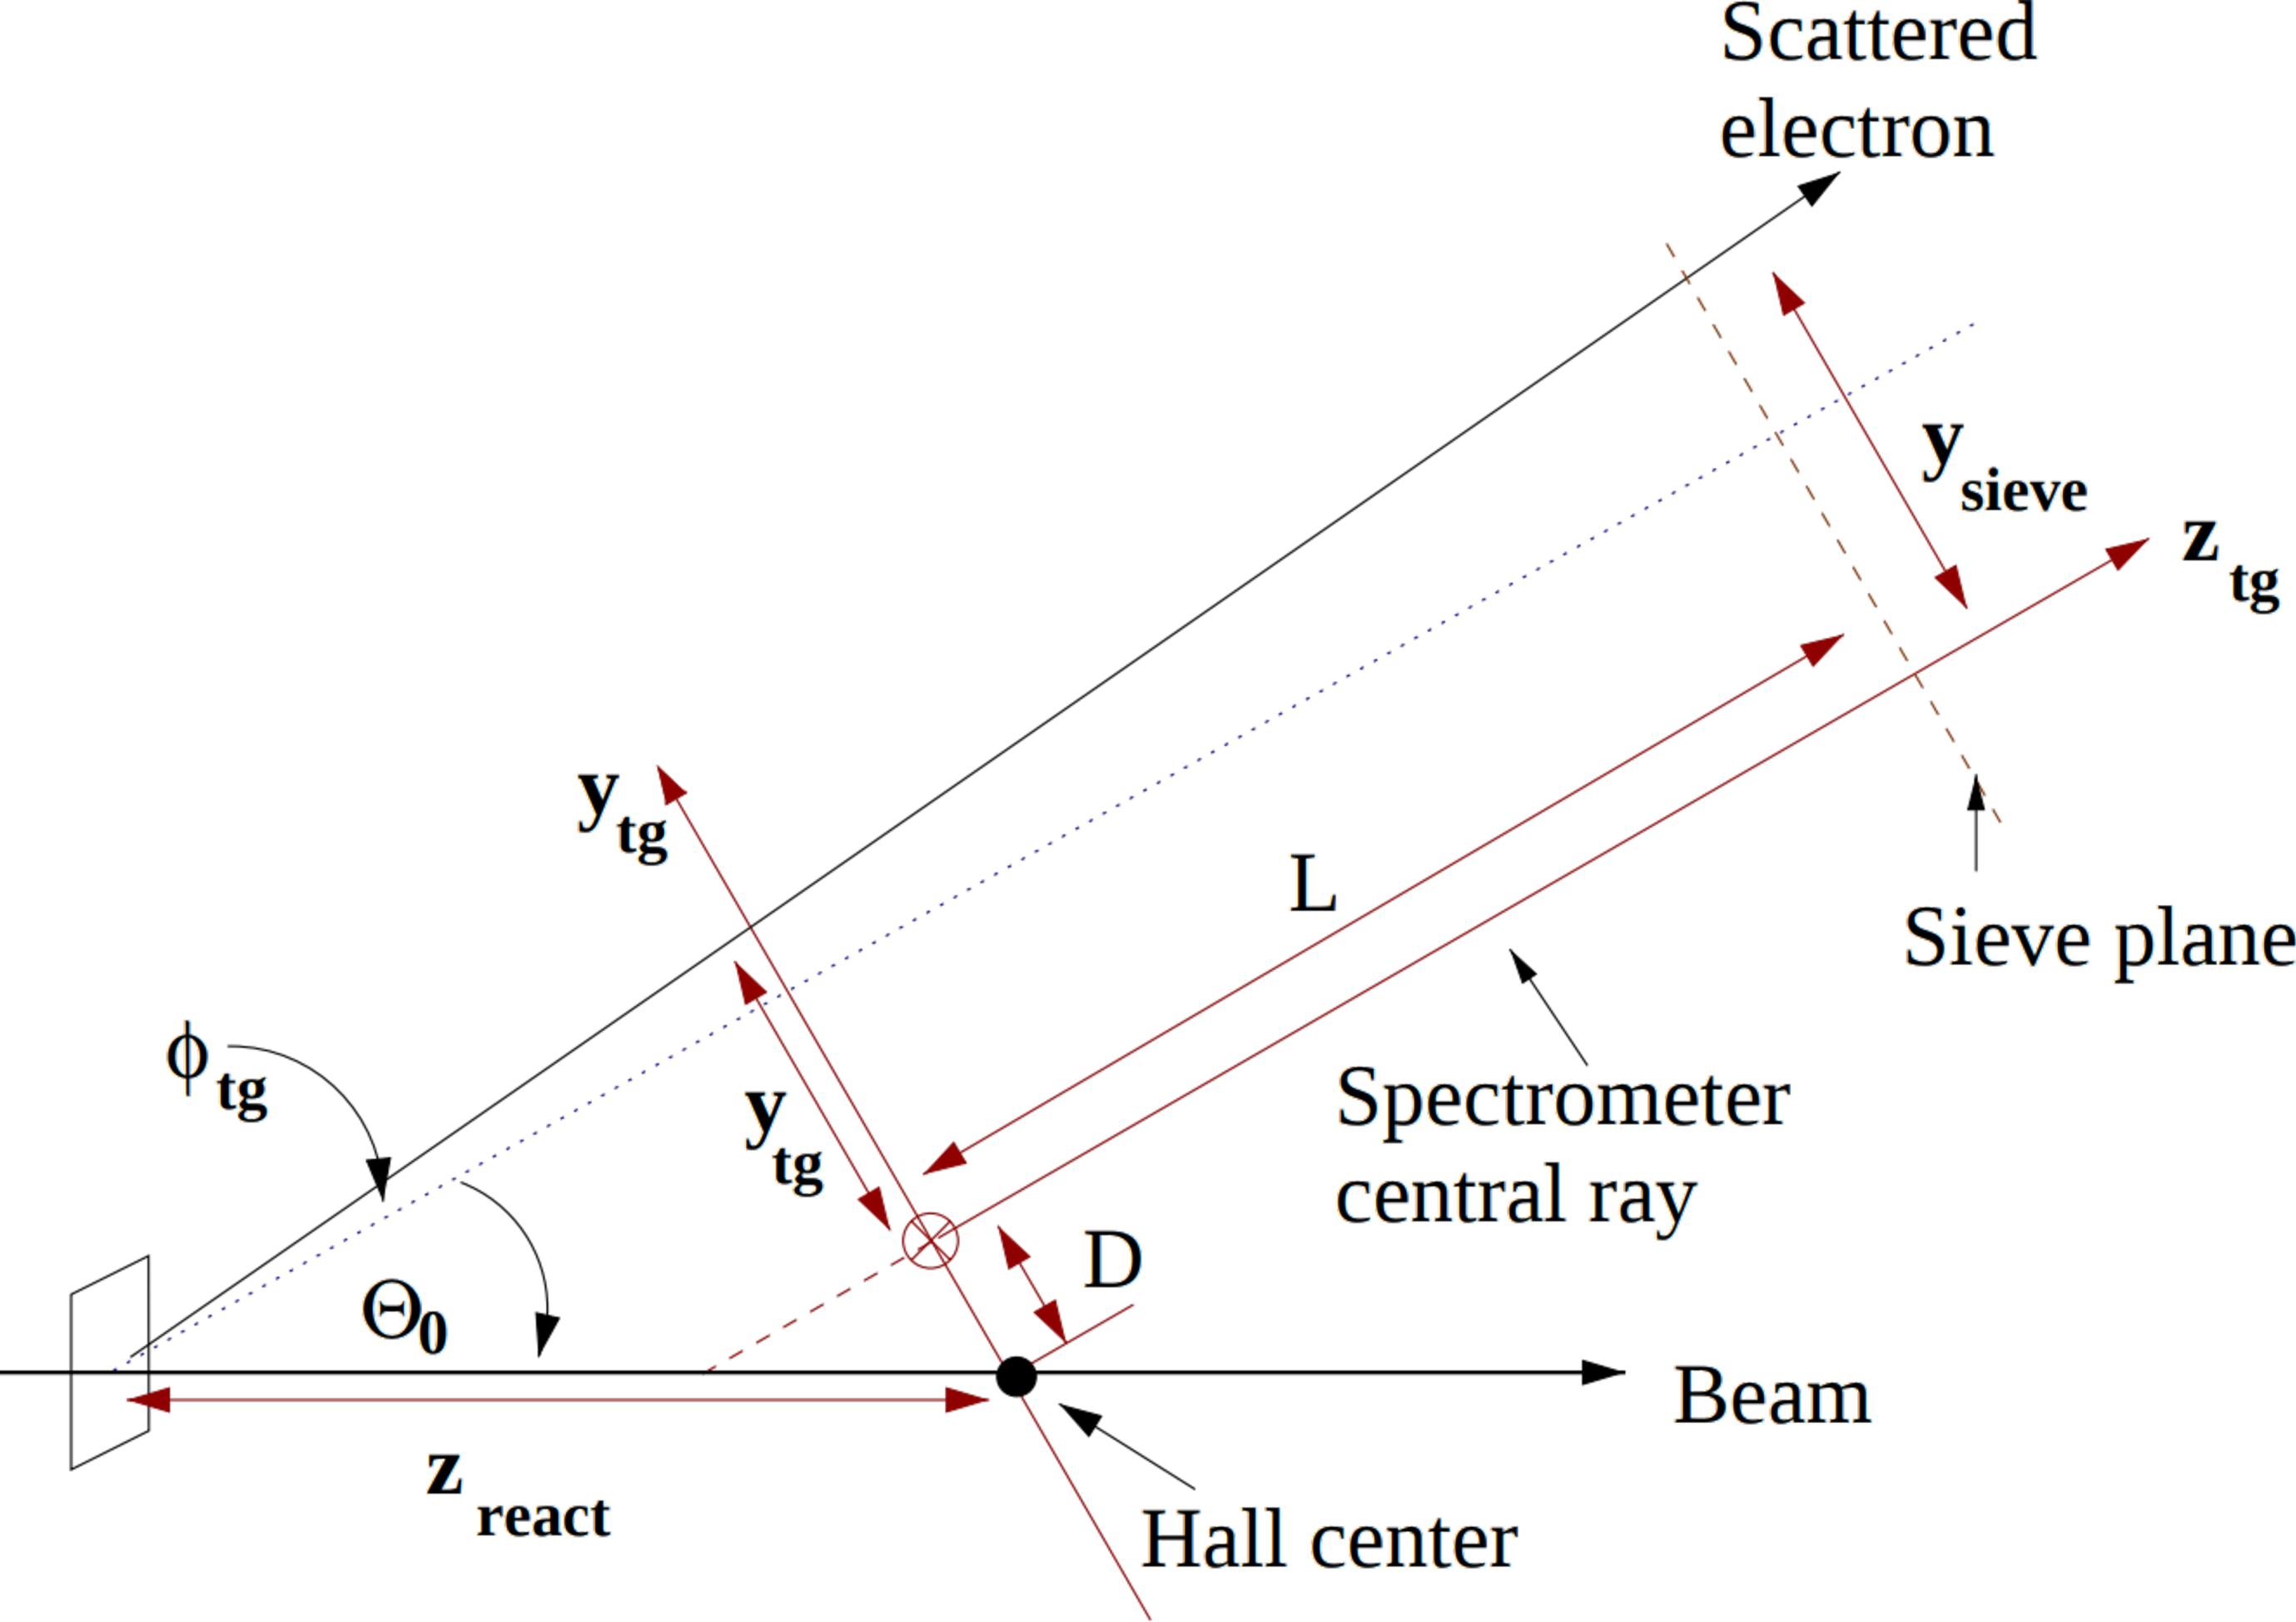
\includegraphics[width=11cm]{TCS.pdf}
		\caption{The TCS for an electron scattering event as seen from above. The event happens at $z_{react}$ distance from the Hall center. \textbf{L} is the distance from the Hall center to the sieve plane. \textbf{D} is the horizontal displacement of the spectrometer axis from the ideal position. $\Theta$ is the spectrometer's central angle. }
		\label{fig:TCS}
	\end{figure}
	\item \textbf{Detector Coordinate System (DCS):}  The origin of the DCS is at the intersection of wire 184 of the U1 and V1 planes of the first VDC. "$\hat{y}$ is parallel to the short symmetry axis of the lower VDC \cite{espace}." $\hat{z}$ is vertically up, perpendicular to the vdc planes.  $\hat{x}$  points away from the center of curvature of the dipole. 
	
\end{itemize}


 

\section{Electron Counting}
\paragraph{}

\section{Efficiencies}
\paragraph{}The high resolution spectrometers are capable of detecting a myriad of particles that track through the detectors. The design of an experimental trigger uses the properties of the individual detectors to capture data of meaningful events. Many accidentals, background, and unwanted events trigger the data acquisition system, and some good electrons are missed by our DAQ. The removal of these unwanted events takes place during analysis via software cuts. Restricting the applicable signal from certain detectors through different cuts allows for the rejection of background particles and prevents contamination in the yield extraction. 

\subsection{Computer and electronic Lifetime}
\paragraph{}The signal from events that fire the DAQ travel through electronics like amplifiers and logic modules on its way to be recorded by the TDCs and ADCs. The processing of these signals require time at each stage. During that time another event will be discarded due to limitations in the hardware. This time when the DAQ system cannot handle another event is known as the dead-time of the system. Lifetime therefor is the percentage of time when an event can be recorded. The lost events need to be account for during the analysis process. The lifetime of the DAQ system for the MARATHON experiment was measured by determining the percentage of events that were recorded relative to the number of events that fired the corresponding trigger. The lifetime for the MARATHON experiment depended on the rate of events. The lifetime during the highest rate kinematic was determine to be 0.947, and climbs to 0.998 for the highest angle setting. Listed in table \ref{LTtable} are the calculated values for lifetime at each kinematic. 

\begin{table}[]
	\textbf{Livetime for each kinematic }\par\medskip
	\begin{tabular}{|l|l|l|l|l|l|l|l|l|l|l|}
		\hline
		Kin      & 1 & 2 & 3 & 4 & 5 & 7 & 9 & 11 & 13 & 15 \\ \hline
		LiveTime & 0.947 & 0.969 & 0.981 & 0.986 & 0.992 & 0.996 & 0.997 & 0.998  & 0.998  & 0.998\\ \hline
	\end{tabular}
	\caption{Livetime during the MARATHON experiment calculated using trigger 2.  }
	\label{LTtable}
\end{table}
  

\subsection{Particle Identification Efficiency}
\paragraph{} One of the largest sources of contamination for the MARATHON experiment are negatively charged pions. These pions are removed through software cuts made in the total signal from the ten cherenkov PMTs(photomultiplier tubes) and the energy deposited into the blocks of both layers of the calorimeter. Electrons can be identified by their behavior in the spectrometer. High-quality electrons will track through the entire detector stack to deposit most of their energy into the total calorimeter system and creating a large amount of light in the cherenkov. Though this knowledge tight cuts can be used to study the efficiency of the particle identification system. Plotting the signal in the cherenkov versus the energy deposited into both layers of the calorimeter allows for visual representation of the sampling cuts made in the efficiency studies, which can be seen in figure \ref{elesample}. 
\begin{equation}\label{effequ}
\begin{split}
GE_{sample} & = \textrm{Known electron sample from tight cut}  \\
GE_{pass} & = \textrm{$GE_{sample}$ and pass indentification cut} \\
Electron_{eff}  & = \frac{ GE_{pass} } { GE_{sample} } 
\end{split}
\end{equation}
\begin{figure}[]
	\centering
	\textbf{Cherenkov sum versus Total Energy deposited }\par\medskip
	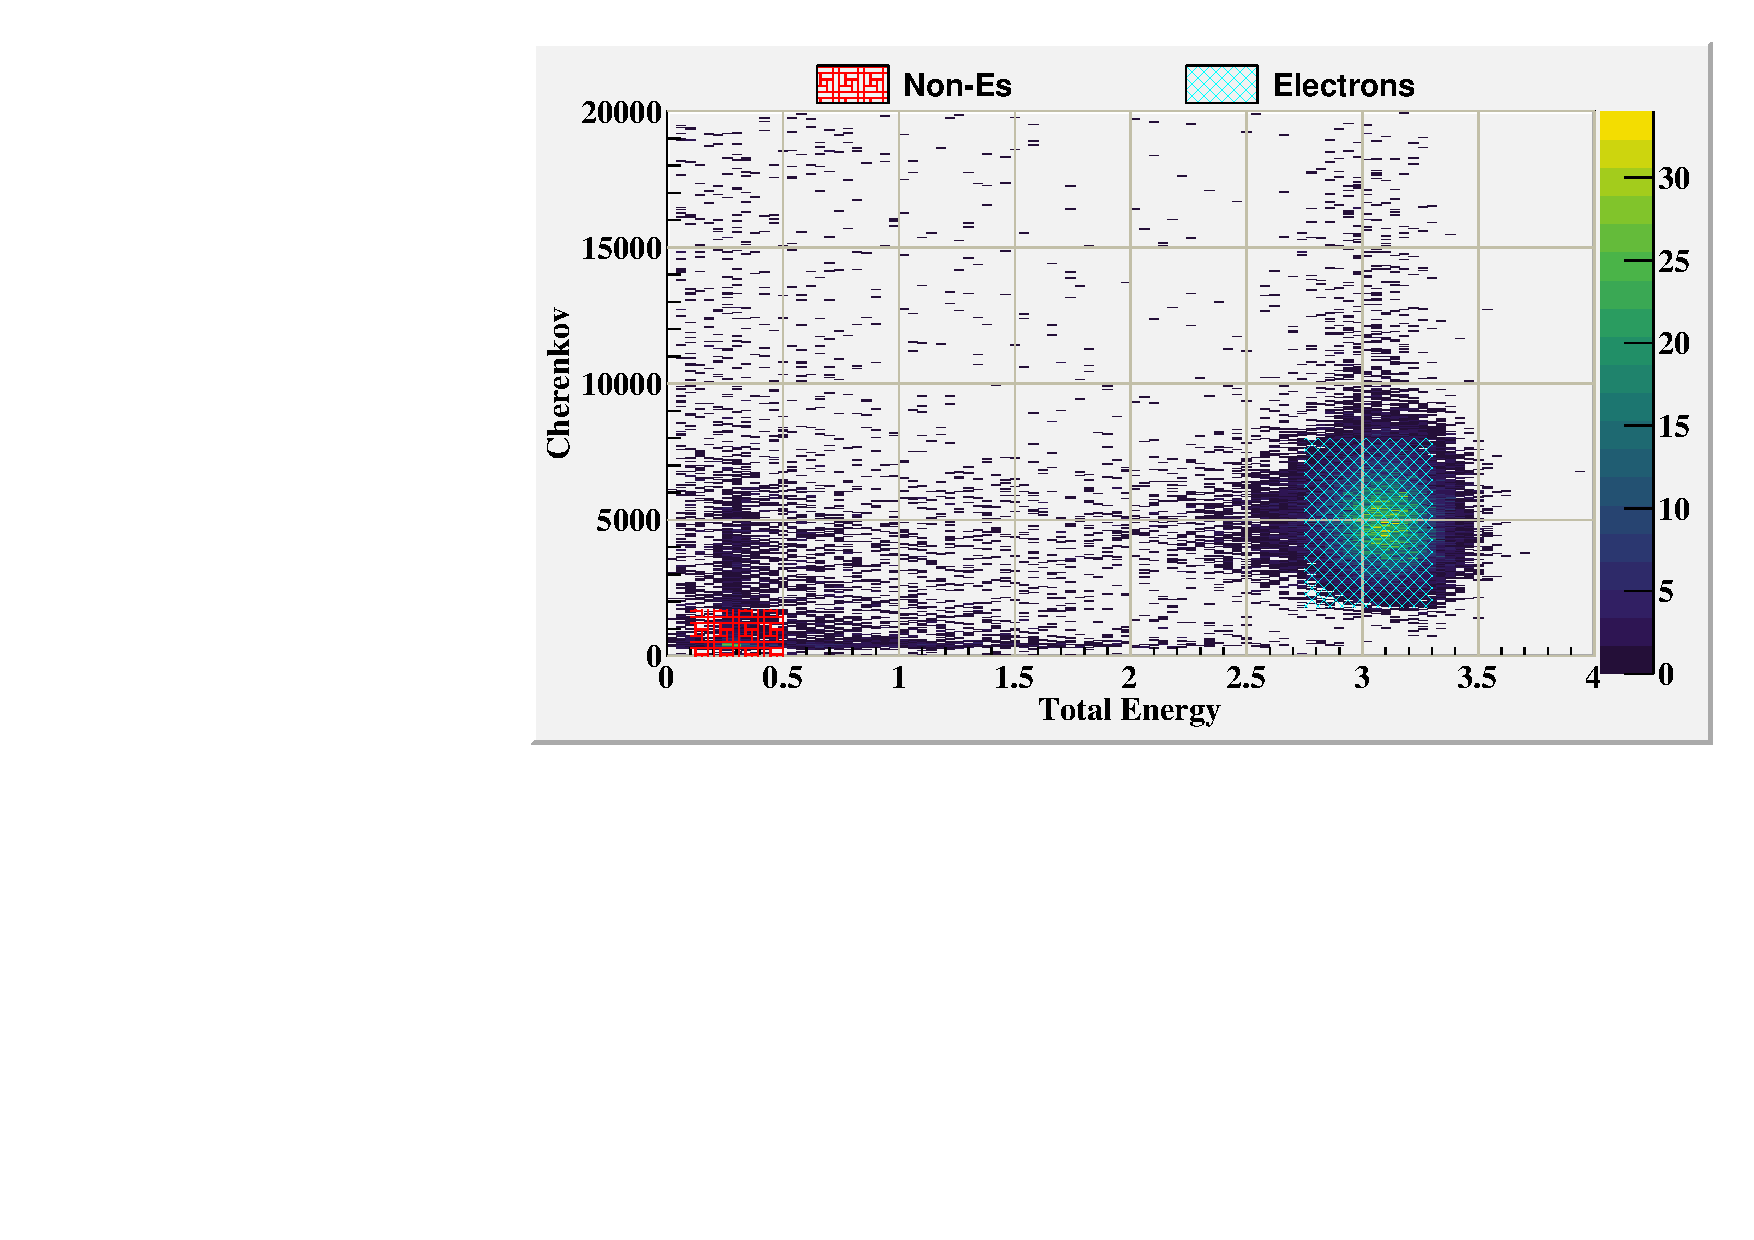
\includegraphics[width=13cm]{PID_2d}
	\caption{Two dimensional plot of the cherenkov sum versus Total Energy deposited, including electron sampling in teal and non-electron sampling in red. }
	\label{elesample}
\end{figure}

\begin{figure}[t]%
	{\centering
		\textbf{Particle ID and efficiency sampling for PID detectors }\par\medskip}
	\centering
	\subfloat[]{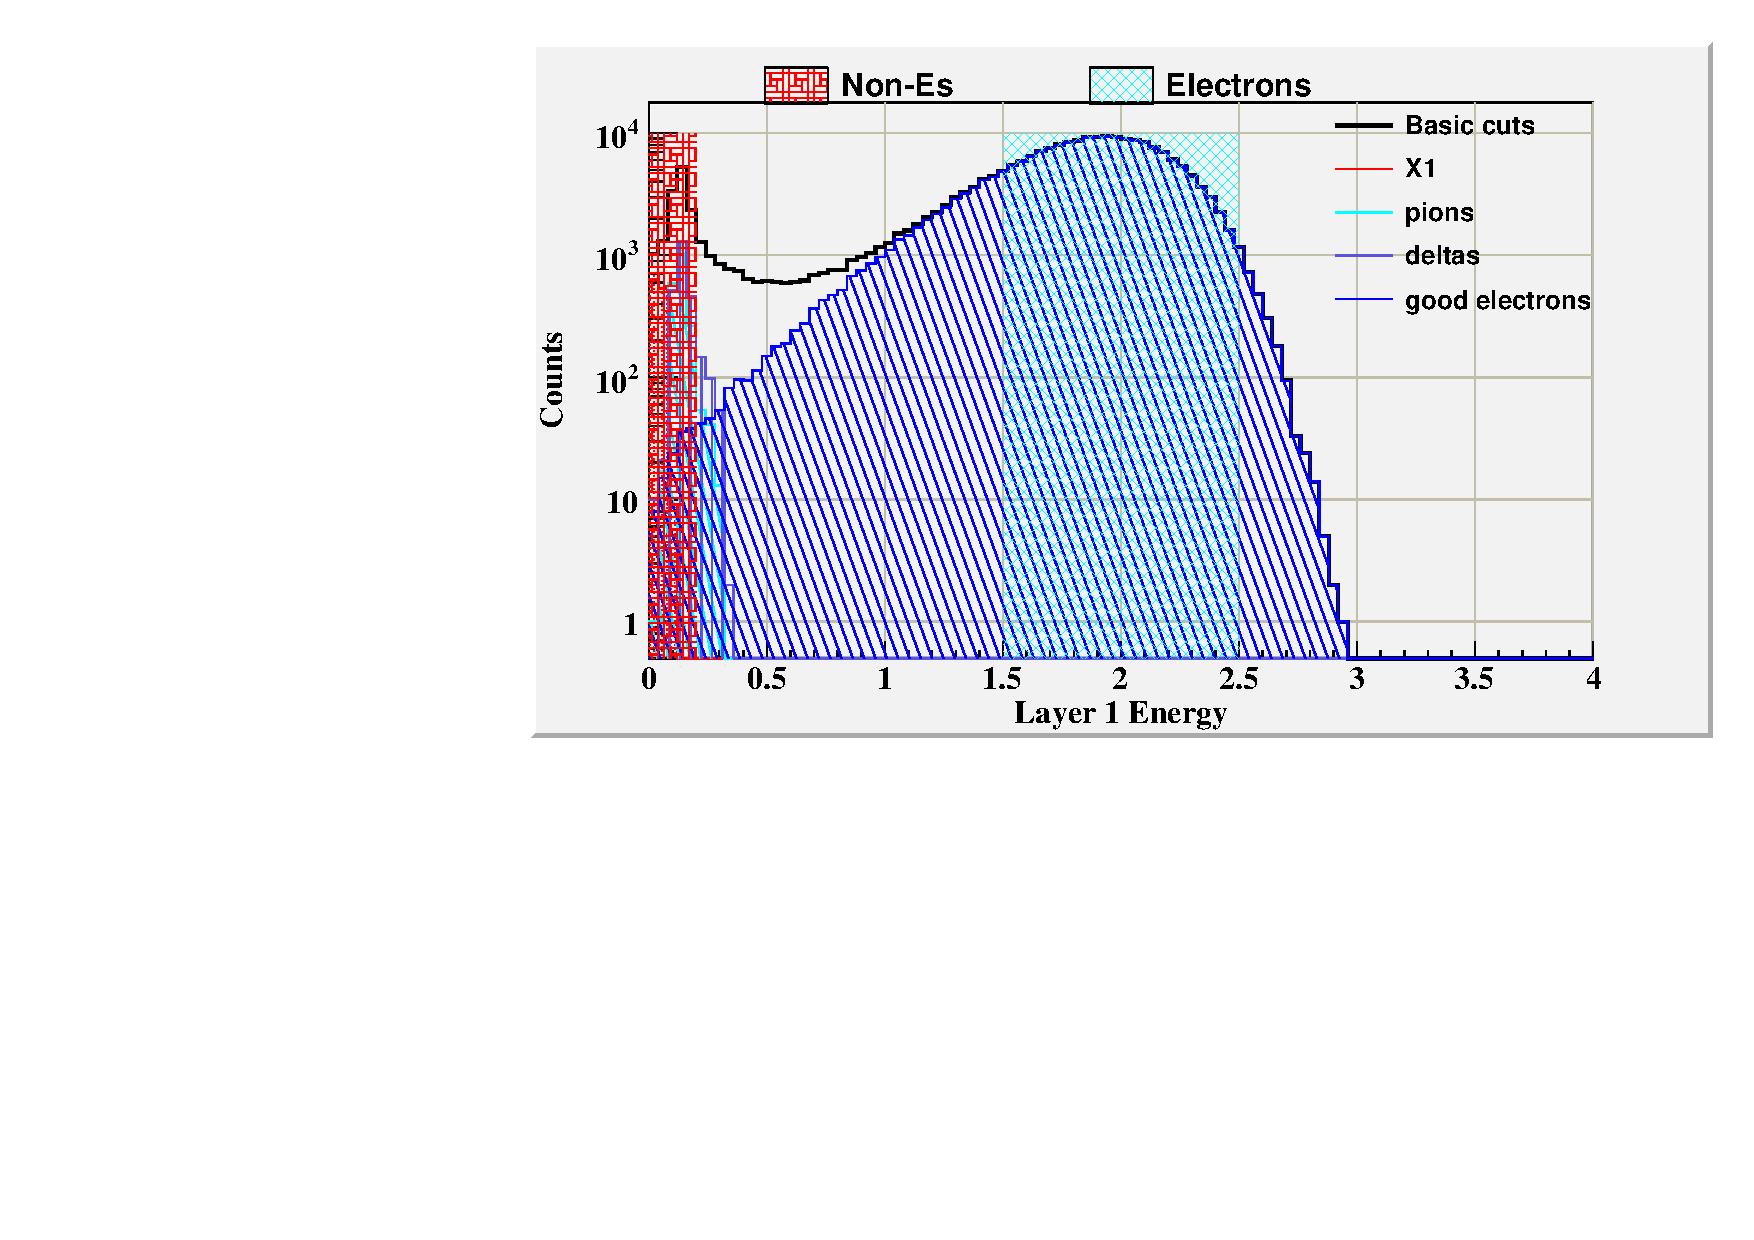
\includegraphics[width=0.5\textwidth,height=4.5cm]{Lprl1}\label{samA}}%
	\subfloat[]{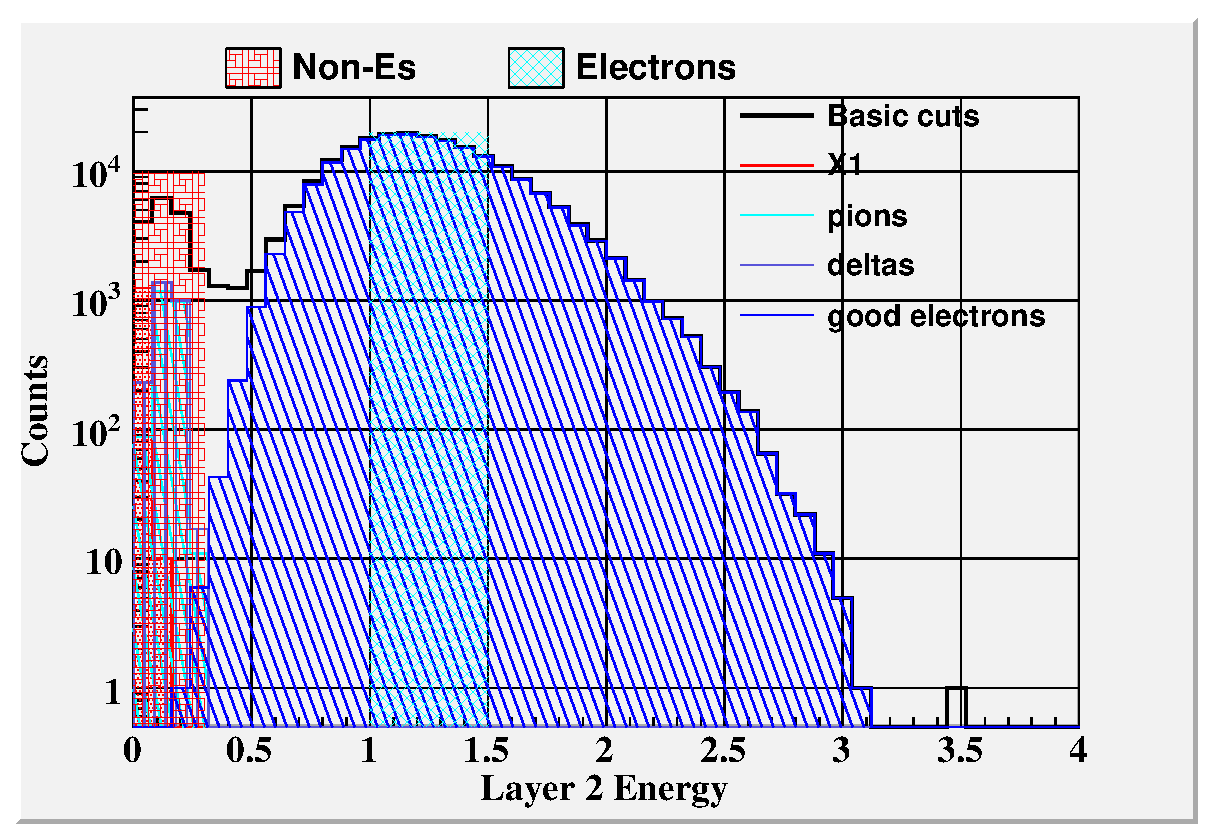
\includegraphics[width=0.5\textwidth,height=4.5cm]{Lprl2}\label{samB}}\\
	\subfloat[]{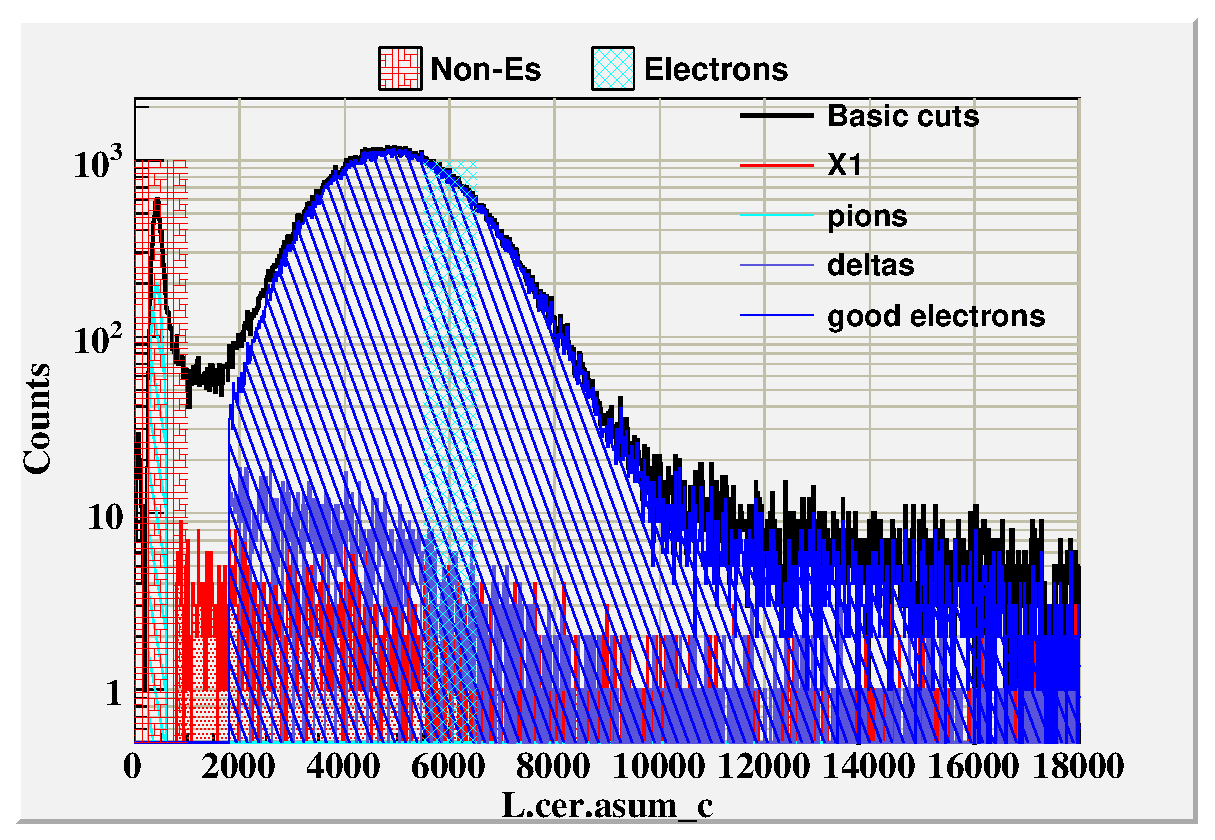
\includegraphics[width=0.95\textwidth,height=3.85cm]{Lcerasum}\label{samC}}%
	\caption{Electrons and other back ground particles identified via cuts in the total calorimeter and the gas cherenkov shown in the individual layers of the calorimeters and the cherenkov. Sampling cuts for Electrons in teal and Non-Electrons in red.}%
	\label{sampling}%
\end{figure}


\paragraph{}The efficiencies of the spectrometer's particle identification(PID) detectors were determined by using the first calorimeter layer, the second calorimeter layer, and the cherenkov to provide samples of good electrons and other particles. The PID efficiency of the individual detectors was determined using equation \ref{effequ}. The good electron sample for calculating the efficiency of the single detector was defined by sampling through the other two detectors. Sampling through the two layers of the calorimeter is shown in figure \ref{samA} for the first layer of the calorimeter and \ref{samB} for the second layer. The cherenkov good electron sample is shown in figure \ref{samC}. The electron sample from the cherenkov is contaminated by delta particles and a combination of unknown particles. These unidentified background particles are known to be relativistic due to the amount of light seen in the cherenkov. However, the events do not deposit enough energy into the calorimeter system to be considered as a good electron that scatter from our target through the detector. Using sampling in one layer of the calorimeter and the cherenkov, these unwanted low energy particles are rejected from sampling for efficiency calculations. The electron selection PID efficiency for the three PID detectors was determine at each kinematic setting to be approximately 98$\%$ . The efficiency was determined to be independent of the kinematic setting. Only small fluctuations were seen during the study, these small changes are due to decrease in statics, and all of the results fall within statical uncertainty of being independent of kinematic setting. The non-electron suppression efficiency was determine as part of this PID efficiency study to ascertain how many back ground particles leak into our sample of good electrons after cuts our made. The suppression efficiency of the cherenkov suffered due to the contamination of the relativistic low energy particles. Combining the two calorimeter detectors with the cherenkov increased the overall suppression efficiency for the spectrometer to 99.9$\%$ over the entire kinematic range of the MARATHON experiment. 

\begin{figure}
	{\centering
		\textbf{PID efficency for each detector for all kinematics. }\par\medskip}
	\centering
	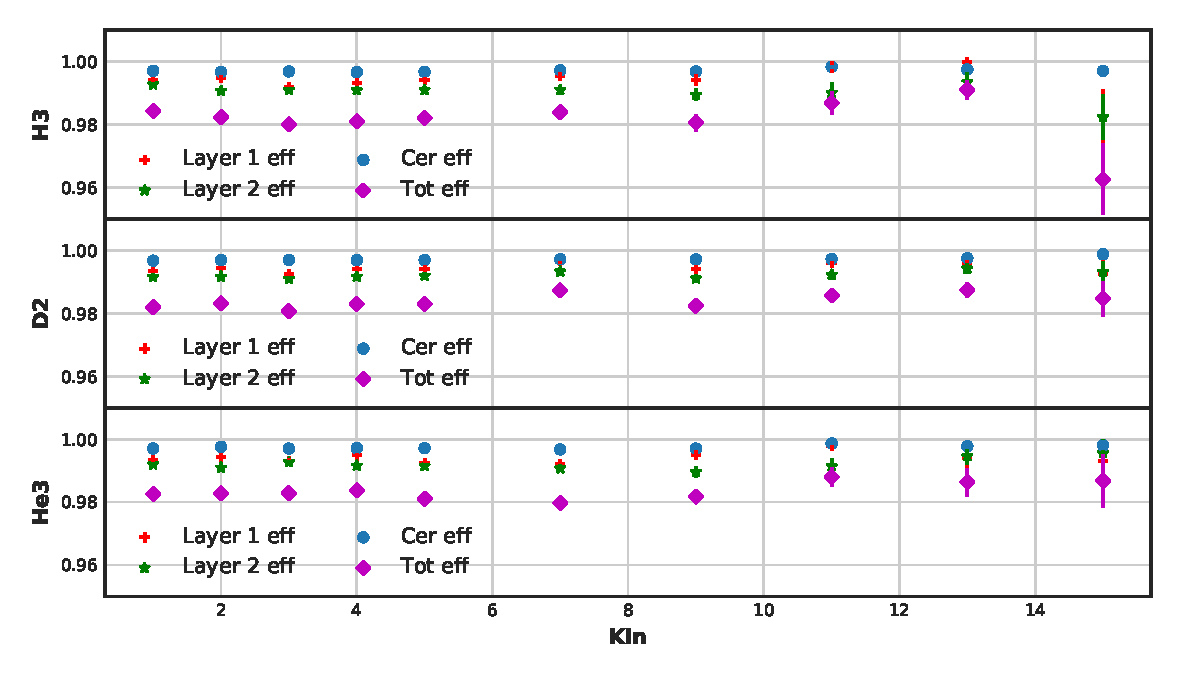
\includegraphics[width=15cm]{PID_allkin_alltgt}
	\caption{The PID efficiency for the cherenkov and both layers of the calorimeter,including the overall total PID efficiency for each of the gas targets at all of the kinematics.}
\end{figure}

\subsection{Trigger Efficiency}
\paragraph{} The process of capturing data from the two HRSs begins with the firing of a trigger. The trigger design for MARATHON focused on triggering for electrons and reducing the amount of other particles. Figure \ref{fig:trig_layout} describes the design of MARATHON's main trigger and efficiency triggers. MARATHON's main trigger, trigger 2, consist of a $(So \& S2) \& Cer$. Due to inefficiencies of the electronics, logic, and detectors an event can produce a false trigger or a high quality electron may not fire 
the main trigger.

\begin{figure}[]
	\centering
	\textbf{Trigger efficiency for the MARATHON experiment }\par\medskip
	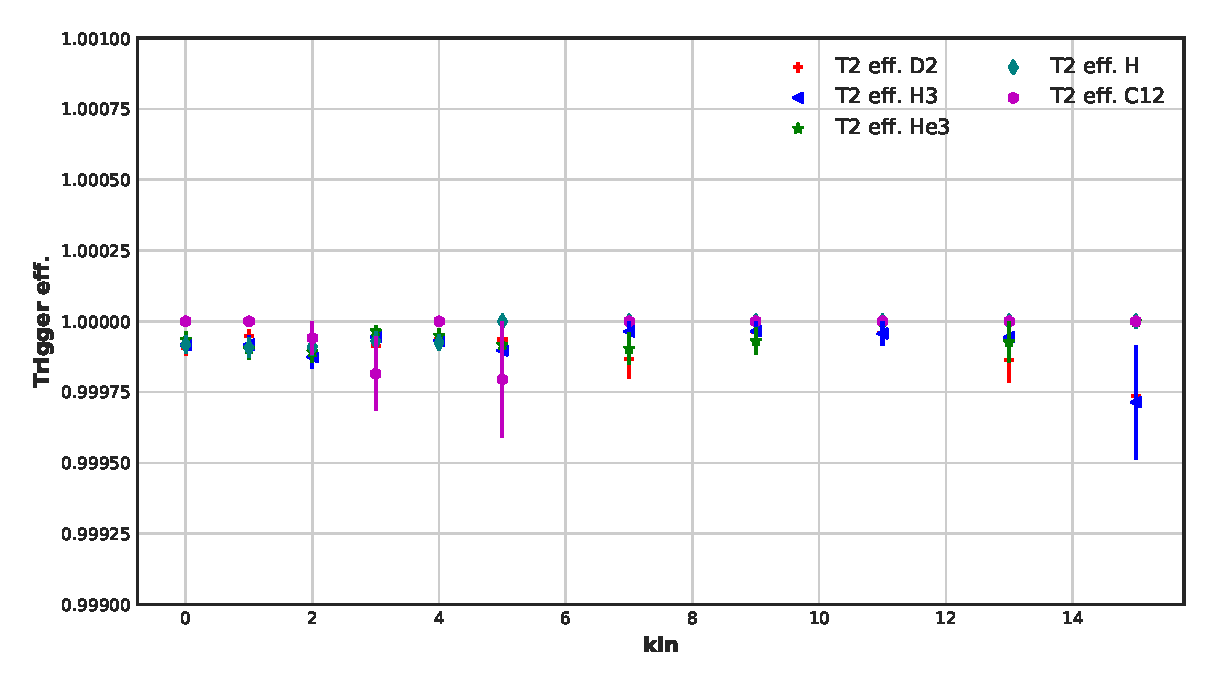
\includegraphics[width=14cm]{Trigger_Eff.eps}
	\caption{Trigger efficiency of trigger 2 for different targets at all kinematics calculated via sampling from trigger 1. }
	\label{trigeff}
\end{figure}

\paragraph{} A low threshold in the cherenkov allows for an inclusive trigger limiting the overall number of quality electrons missed, but allows for a large quantity of false triggers. Software PID cuts prevent the contamination of false positives from trigger inefficiencies. The tight PID software cuts removes the false positive inefficiency from the trigger design and is then considered in the PID efficiencies. The trigger inefficiency caused by missed high quality electrons was then calculated by sampling the high quality electrons in trigger 1, $(S_o \& S_2)$. This ties the efficiency of trigger 2 with the performance of the scintillators. The efficiency of the two scintillating planes in conjunction is calculated by using sampling in trigger 3, $(S_o | S_2) \& Cer$ with strict PID cuts in both layers of the calorimeters and requiring a hit in the cherenkov. The two scintillator planes in conjunction have an efficiency greater than $99.7 \% $ for all kinematics. Combining the trigger efficiency of the main trigger shown in figure \ref{trigeff} with the performance of the scintillators give an over all efficiency for the trigger of the MARATHON experiment of greater then $99.6\%$.

\subsection{Tracking Efficiency}
\begin{figure}[]
	\centering
	\textbf{Tracking efficiency for the MARATHON experiment }\par\medskip
	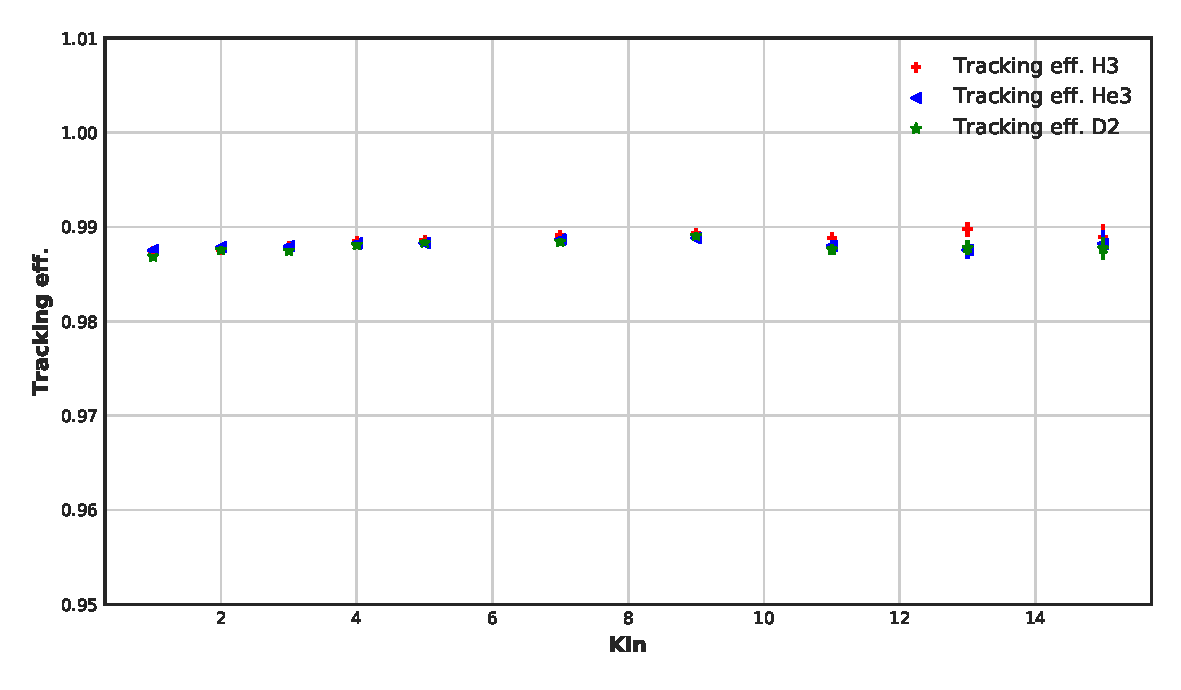
\includegraphics[width=15cm]{Tracking_Eff_allkin.eps}
	\caption{Tracking efficiency of the VDCs for different targets at all kinematics. }
	\label{trackeff}
\end{figure}
\paragraph{}Particles that travel through our detector could originated from sources wanted or unwanted. In order to control the source of the scatter electrons, we use a particle's track to identify its source. The signals received via the VDC is used to produce a particles track from the target to end of the spectrometer. The largest source of inefficiency for the VDCs are incorrectly identified tracks. High quality electrons that transverse the spectrometer should only have one good track, calculated via the tracking package in the analysis software. The capability of the VDCs to determine a good electron event's one good track is know as the one track efficiency for the VDCs. Quantitatively the one track efficiency ($\epsilon_{VDC}$) can be obtained via:
\begin{equation}
\epsilon_{VDC} \equiv \frac{N_{1 track} }{N_{all}}
\end{equation}
Where the number of good electron events that have one good track is defined as $N_{1 track}$, and $N_{all}$ are all of the electrons rather they have a good track or not. The good electron selection is made via PID cuts in the calorimeter and cherenkov, and cuts in the ADC and TDC of the scintillators. Direct cuts in the signal of the scintillators where made to include the nominal acceptance cuts, which our produced through tracking software. The tracking efficiency of HRSs during the MARATHON experiment is shown in figure \ref{trackeff} for the three gas targets during all kinematic ranges. The efficiency of the VDCs is not relative to the angle of the spectrometer. So the uniform tracking efficiency across all kinematics is expected and helps eliminate any concerns of the performance of the VDCs during the experiment. 

\section{Background Subtraction}
\paragraph{} The purpose of this analysis is to study the DIS cross sections of deuterium, helium-3, and tritium. The sample of scattered events used to determine the cross section of a given nuclear target then needs to be cleaned of any contamination produced from other targets and processes. The electrons detected by the spectrometers can be electrons that scatted from our chosen target, scattered from a source other then our target, or produced through process other than DIS scattering. The two sources of contamination for the MARATHON experiment are events scattered from the aluminum end caps of the target cell and pair produced electrons via photon interaction. 
\subsection{End Caps}
\paragraph{} The target cells used during the MARATHON experiment are shown in figure \ref{HATT}. The majority of the events from the end caps can be removed easily via a cut in the reconstructed quantity of reaction vertex along the beam axis. The relatively large density thickness of the aluminum end caps cause a large amount of end cap contamination. The majority of the electrons that scatter from the end caps can be removed through software cuts in the reaction vertex along the beam axis(z). Show in figure \ref{EC5} is a comparison of the reaction vertex of the electron events between the gaseous targets and the empty cell target at kinematic 4. The yield is normalized by the number of event in the histogram to remove any bias from the amount of time of beam on target. The empty target  results in figure \ref{EC5}, demonstrate the form of scattering off of the aluminum windows of our target cell. Using the reconstructed vertex location of the scattering origin, the vast majority of the events from the windows can be removed. This vertex cut is shown by the two vertical blue lines. Only events that lie within these two line are considered good electrons from our chosen target. 


\begin{figure}[]
	\centering
	\textbf{Scattering vertex along the beam axis. }\par\medskip
	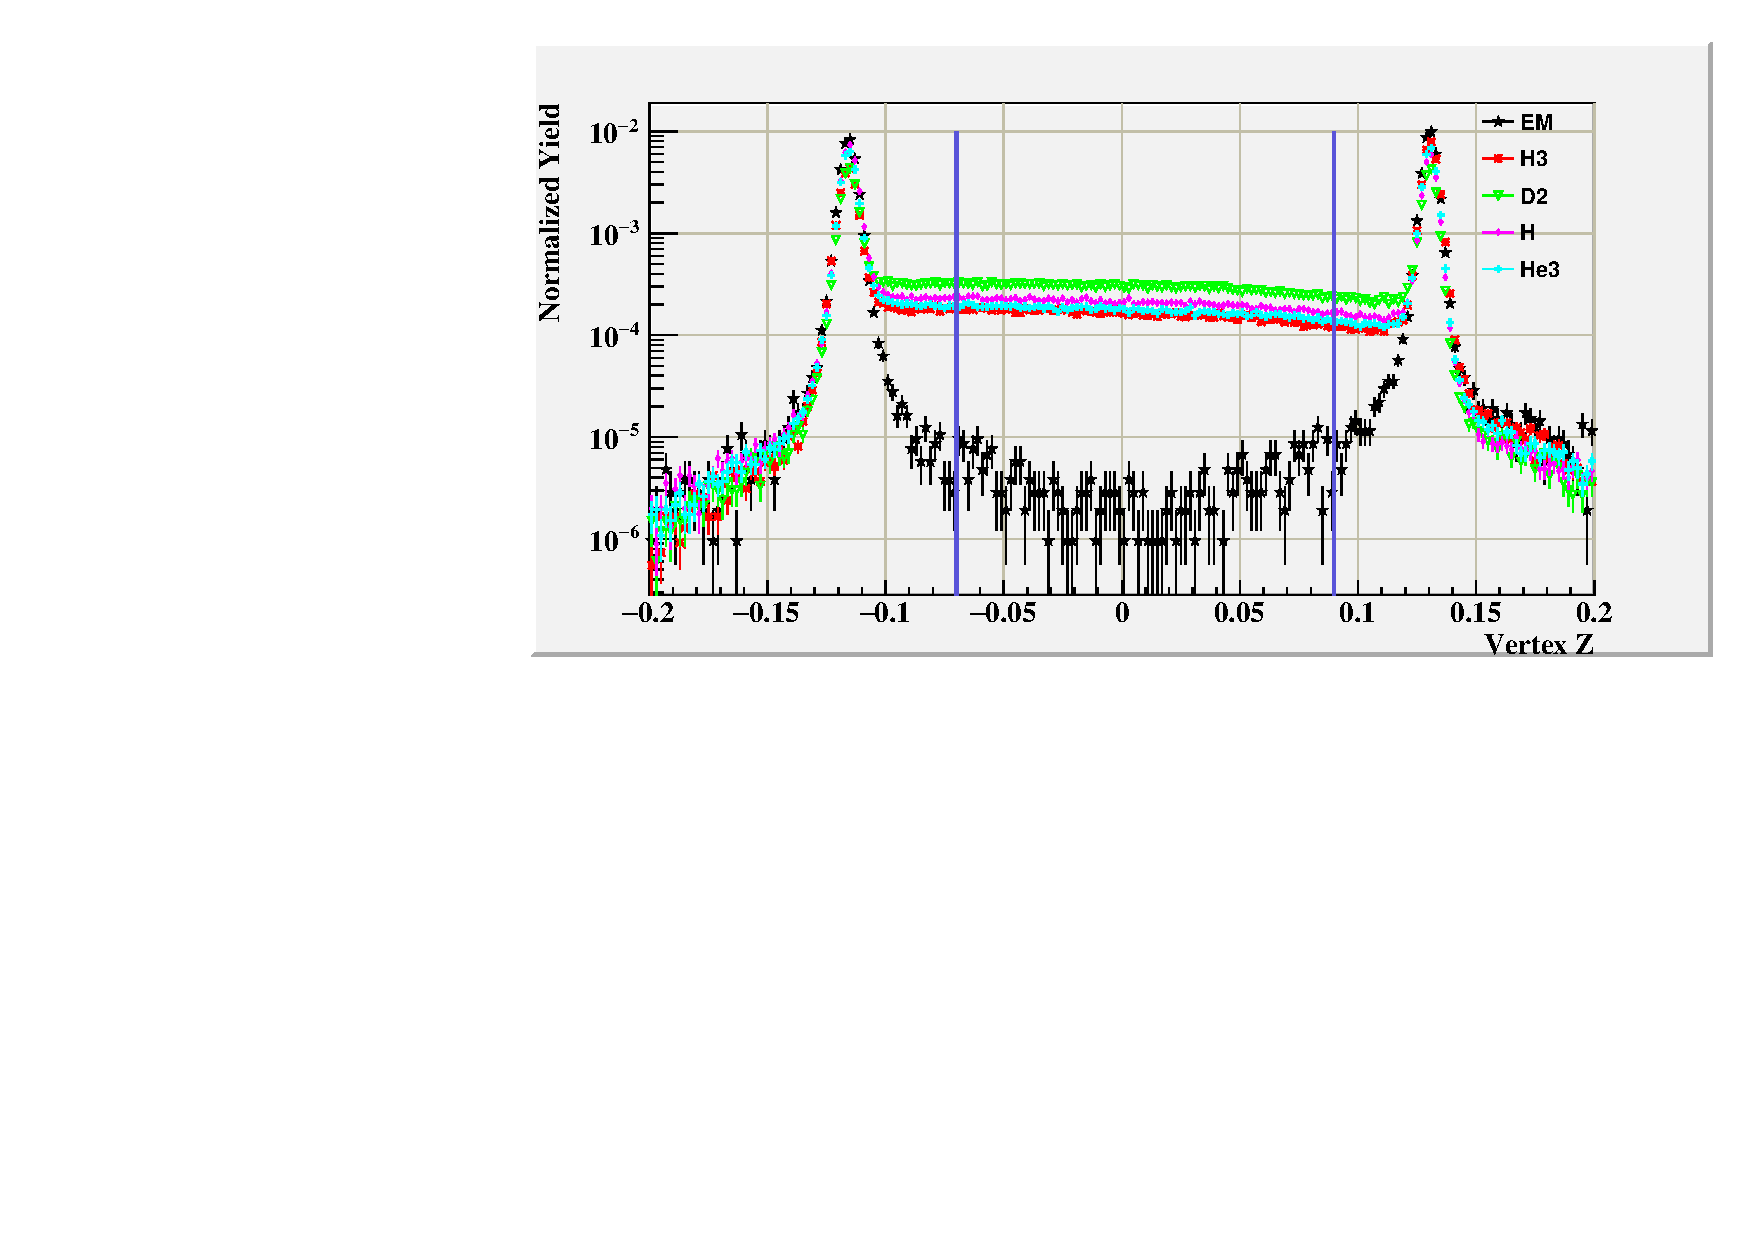
\includegraphics[width=15cm]{endcap_kin4.pdf}
	\caption{Comparison of the scattering vertex along the z axis for the empty target(EM) and the gas targets at kin. 4. }
	\label{EC5}
\end{figure}

\paragraph{}The empty cell vertex z disruption does have content within the vertex cut. These events that remain after the cut are corrected for via an end cap contamination factor. This  factor is calculated by determining the ratio of the number of good electrons that scatter from the empty cell and from each gas cells, resulting in ratio of $\big(\frac{Yield_{EC}}{(Yield_{Gas} + Yield_{EC})}\big)$. Where the subscript EC denotes events from the end caps. The correction factor applied to the yield calculation is defined as:
\begin{equation*}
ECC = 1- \big(\frac{Yield_{EC}}{(Yield_{Gas} + Yield_{EC})}\big) \equiv \frac{Yield_{gas}}{(Yield_{Gas} + Yield_{EC})}
\end{equation*}

%\begin{table}[]
%	\textbf{End cap contamination for each target at all kinematics. }\par\medskip
%	\hspace{-70pt}
%	\begin{tabular}{|l|l|l|l|l|l|l|l|l|l|l|}
%		\hline
%		Kinematic  & 1       & 2       & 3        & 4        & 5        & 7       & 9       & 11       & 13       & 15   \\ \hline
%		H3   & 0.0218 & 0.0202 & 0.0163   & 0.0154   & 0.01445  & 0.01177 & 0.009   & 0.0069   & 0.0055   & 0.0043     \\ \hline
%		He3  & 0.0251 & 0.0229 & 0.01839  & 0.01727  & 0.01573 & 0.0125  & 0.00974 & 0.00715  & 0.00572 & 0.00449  \\ \hline
%		D2   & 0.0113 & 0.010  & 0.008206 & 0.00934 & 0.00864  & 0.00831 & 0.0057  & 0.00512 & 0.00379  & 0.00276   \\ \hline
%		H    & 0.0238  & 0.020 & 0.0178   & 0.0176   &          &         &         &          &          &            \\ \hline
%	\end{tabular}
%	\caption{The amount of electrons that scatter from the empty cell compared with the amount electrons that scatter off a gas filled cell. }
%	\label{ECCtable}
%\end{table}



\subsection{Pair Produced Electrons}
\paragraph{} The high energy scattering interaction used to create deep inelastic scattering events can produce high energy photons and pions. The high energy photons that have energy greater than 1.022 MeV can convert into e$^+$e$^-$ pairs when the photons interact with a medium.   
%\begin{figure}[h]
%	\centering
%	\textbf{Pair Production Feynman diagram}\par\medskip
%	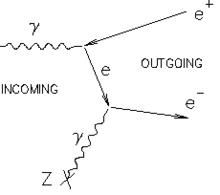
\includegraphics[width=6.0cm]{../images/pp_FD.png}
%	\caption{A feynman diagram of positron electron pair produced via photon interaction.}
%	\label{PC_fey}
%\end{figure}
A correction for the number of back ground electrons produced via a pair production process was calculated by determining the amount of positrons produced from equal targets and kinematics. The yield of positrons were measured for kinematics one through five. The results were used to construct a function to determine the amount of contamination at high $x_{Bj}$ kinematics. Figure \ref{PC} shows the amount of positron contamination for tritium and an exponential fit to extrapolate over the entire ranged in $x_{Bj}$ for the MARATHON experiment. 

\begin{figure}[h]
	\centering
	\textbf{Tritium positron contamination. }\par\medskip
	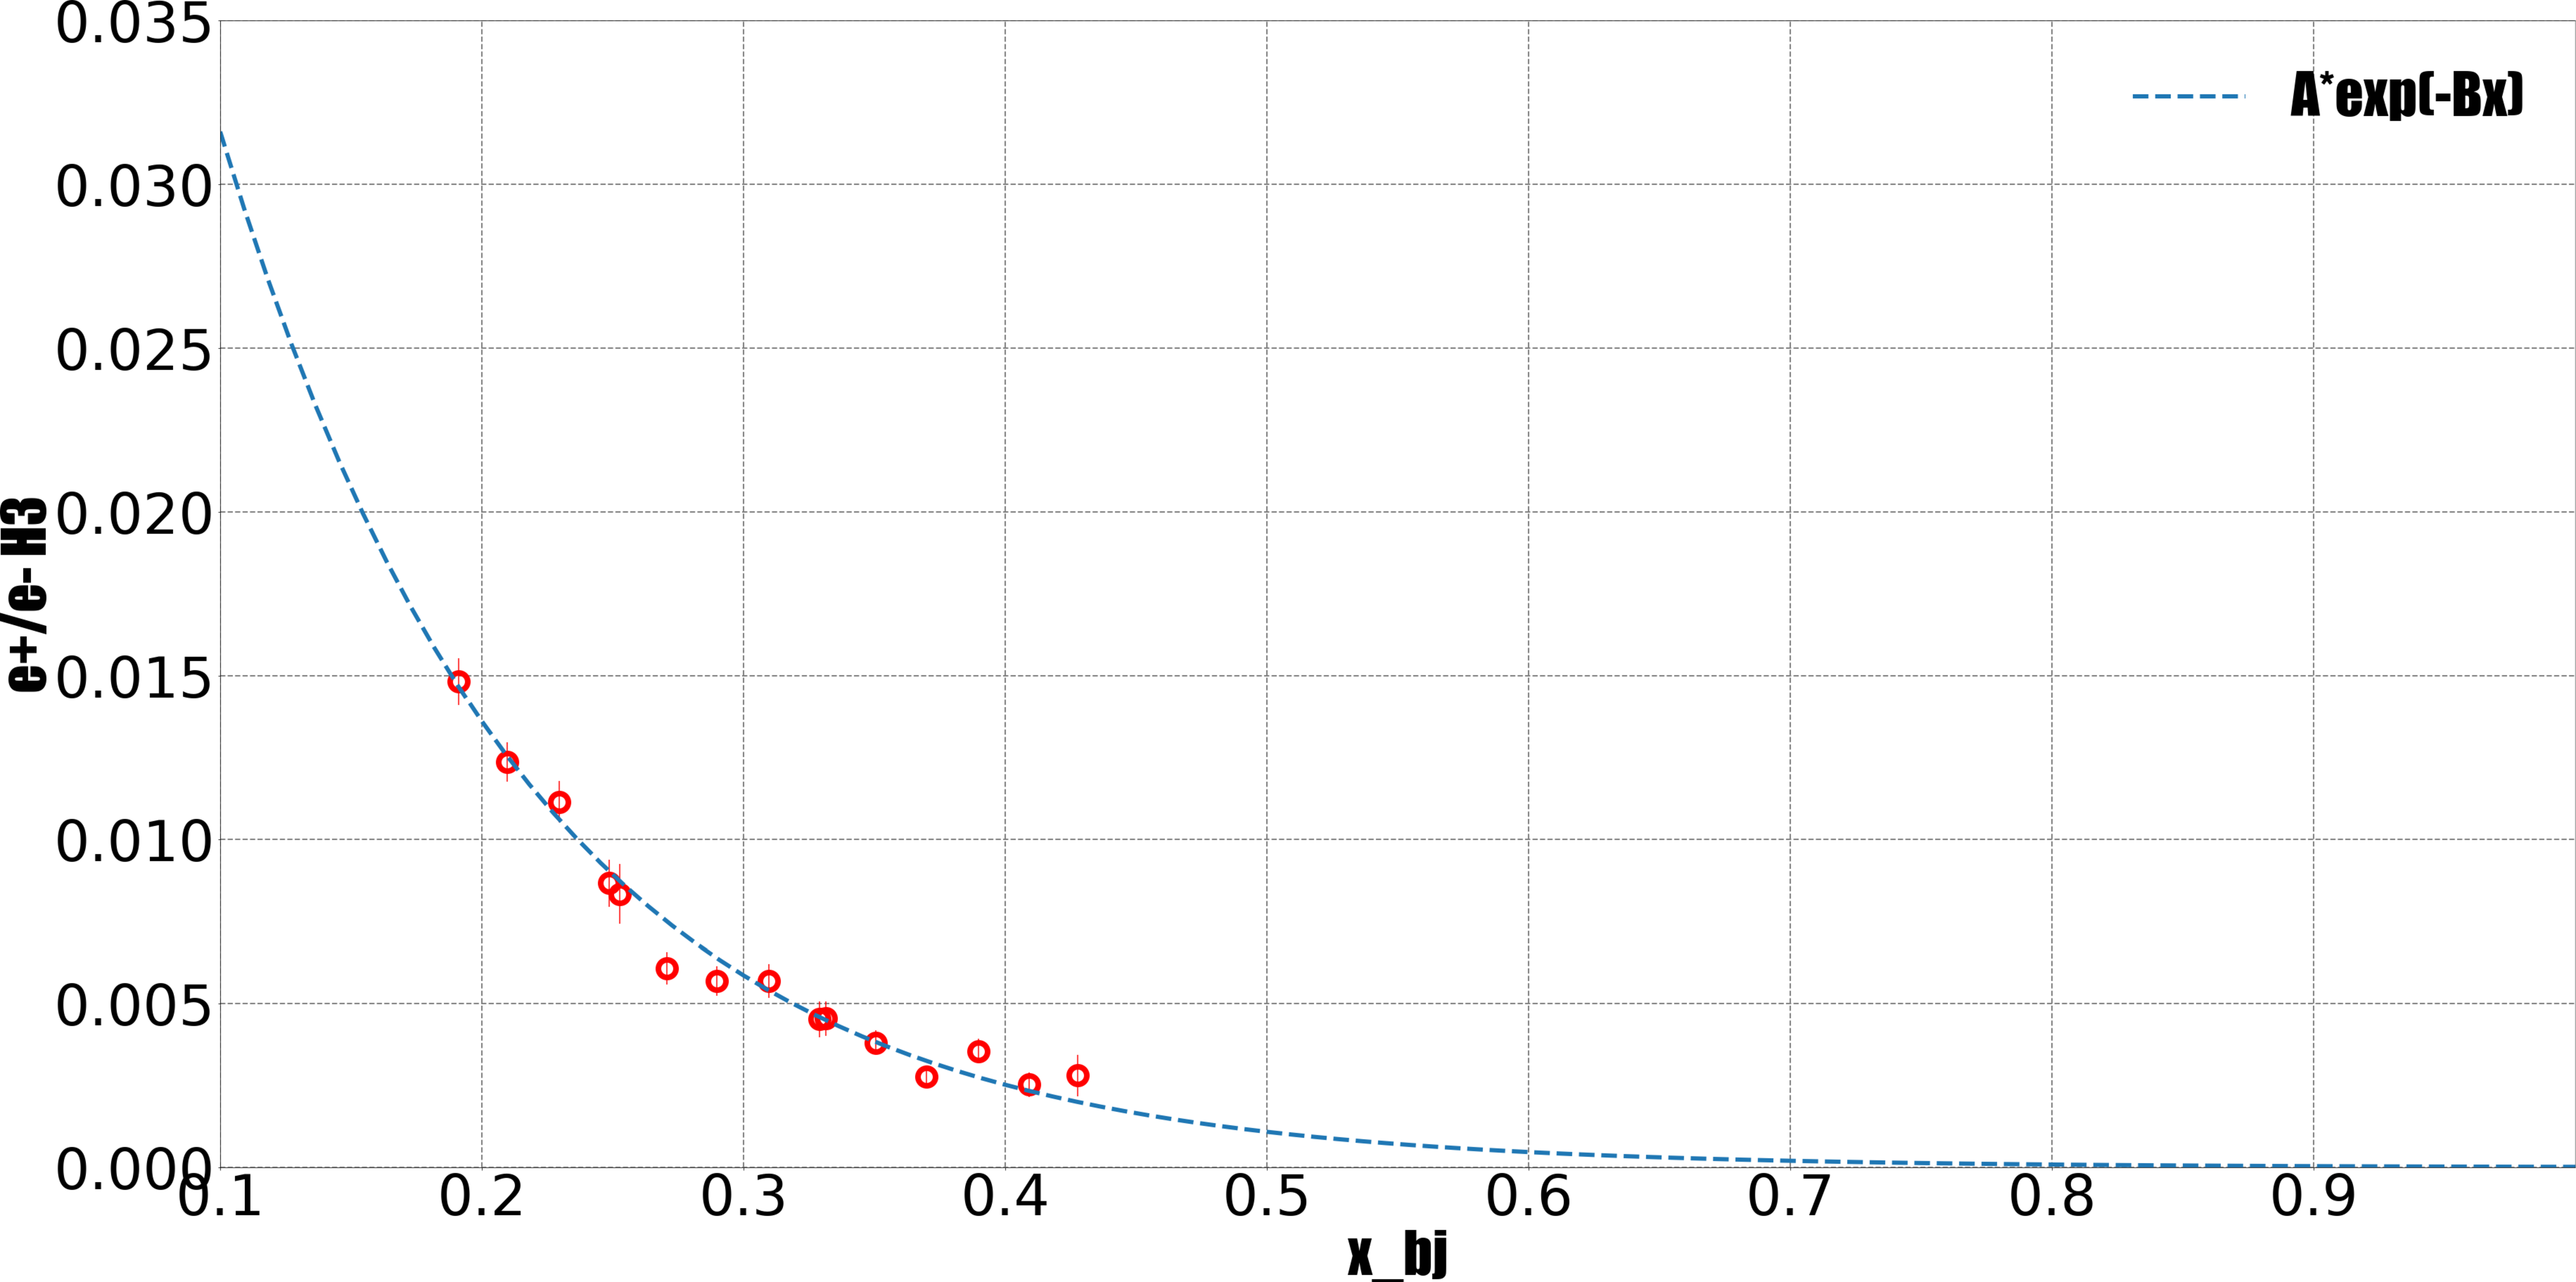
\includegraphics[width=15.0cm]{../images/positron_H3_bane.pdf}
	\caption{The ratio of positron events to electrons for tritium \cite{tongsu}. }
	\label{PC}
\end{figure}


\subsection{Beta Decay of Tritium}
\paragraph{} Tritium a radioactive isotope of hydrogen will beta decay to $^3$He. Tritium has a half-life of 4500 $\pm$ 8 days \cite{T2HL}. The gas cell used to contain Tritium for the experiment was filled on October 23, 2017. The initial tritium thickness density of our tritium cell was $0.077 \pm 0.001 $ grams per cm$^2$. Tritium will decay to $^3$He via a beta interaction. The tritium in our cell is diatomic and decays via two channels\cite{diaT}. The possible decay channels and their branching probabilities are shown in equation \ref{branching}. In DIS interactions, the molecular effects are ignored due to the size of the probe in a DIS scattering event which allows for the different channels to be treated as one. 
\begin{align}
			^3H_2 &\rightarrow(^3H ^3He)^+  &(94.5 \pm 0.6\%) \nonumber \\ 
			^3H_2 &\rightarrow(^3H)^+ + (^3He)^+  & (5.5 \pm 0.6\%) 
			\label{branching}
\end{align}
\paragraph{}The amount of $^3$H and $^3$He in our tritium cell will change in respect to the time since the feeling of the cell. Equations \ref{nT} and \ref{nH} describe the amount of $^3$H and $^3$He in the tritium cell has a function of the time since fill date and the original amount of $^3$H and $^3$He in cell at filling. In equations \ref{nT} and \ref{nH}, $n_T(n_H)$ is the time dependent amount of tritium(helium), and  $n_T^0(n_H^0)$ is the amount of tritium(helium) in the cell at time of filling. t is the time since the cell was filled and $\tau$ is the mean lifetime of tritium.
\begin{align}
	n_T &= n_T^0 \: e^{-t/\tau} \label{nT}\\
	n_H &= n_H^0(1 - e^{-t/\tau}) \label{nH},
\end{align}
As time passes the amount of $^3He$ increases, the contamination becomes a non-negligible effect on the yield of scattered electrons. The fraction of $^3He$ in the tritium can reach up to 3$\%$ for the data from the end of the MARATHON experiment. This $^3He$ fraction as a function of time is shown in figure \ref{Hfract}, with the period for running the MARATHON experiment labeled as a color band. 

\begin{figure}[t]
	\centering
	\textbf{Helium Fraction from Tritium Cell. }\par\medskip
	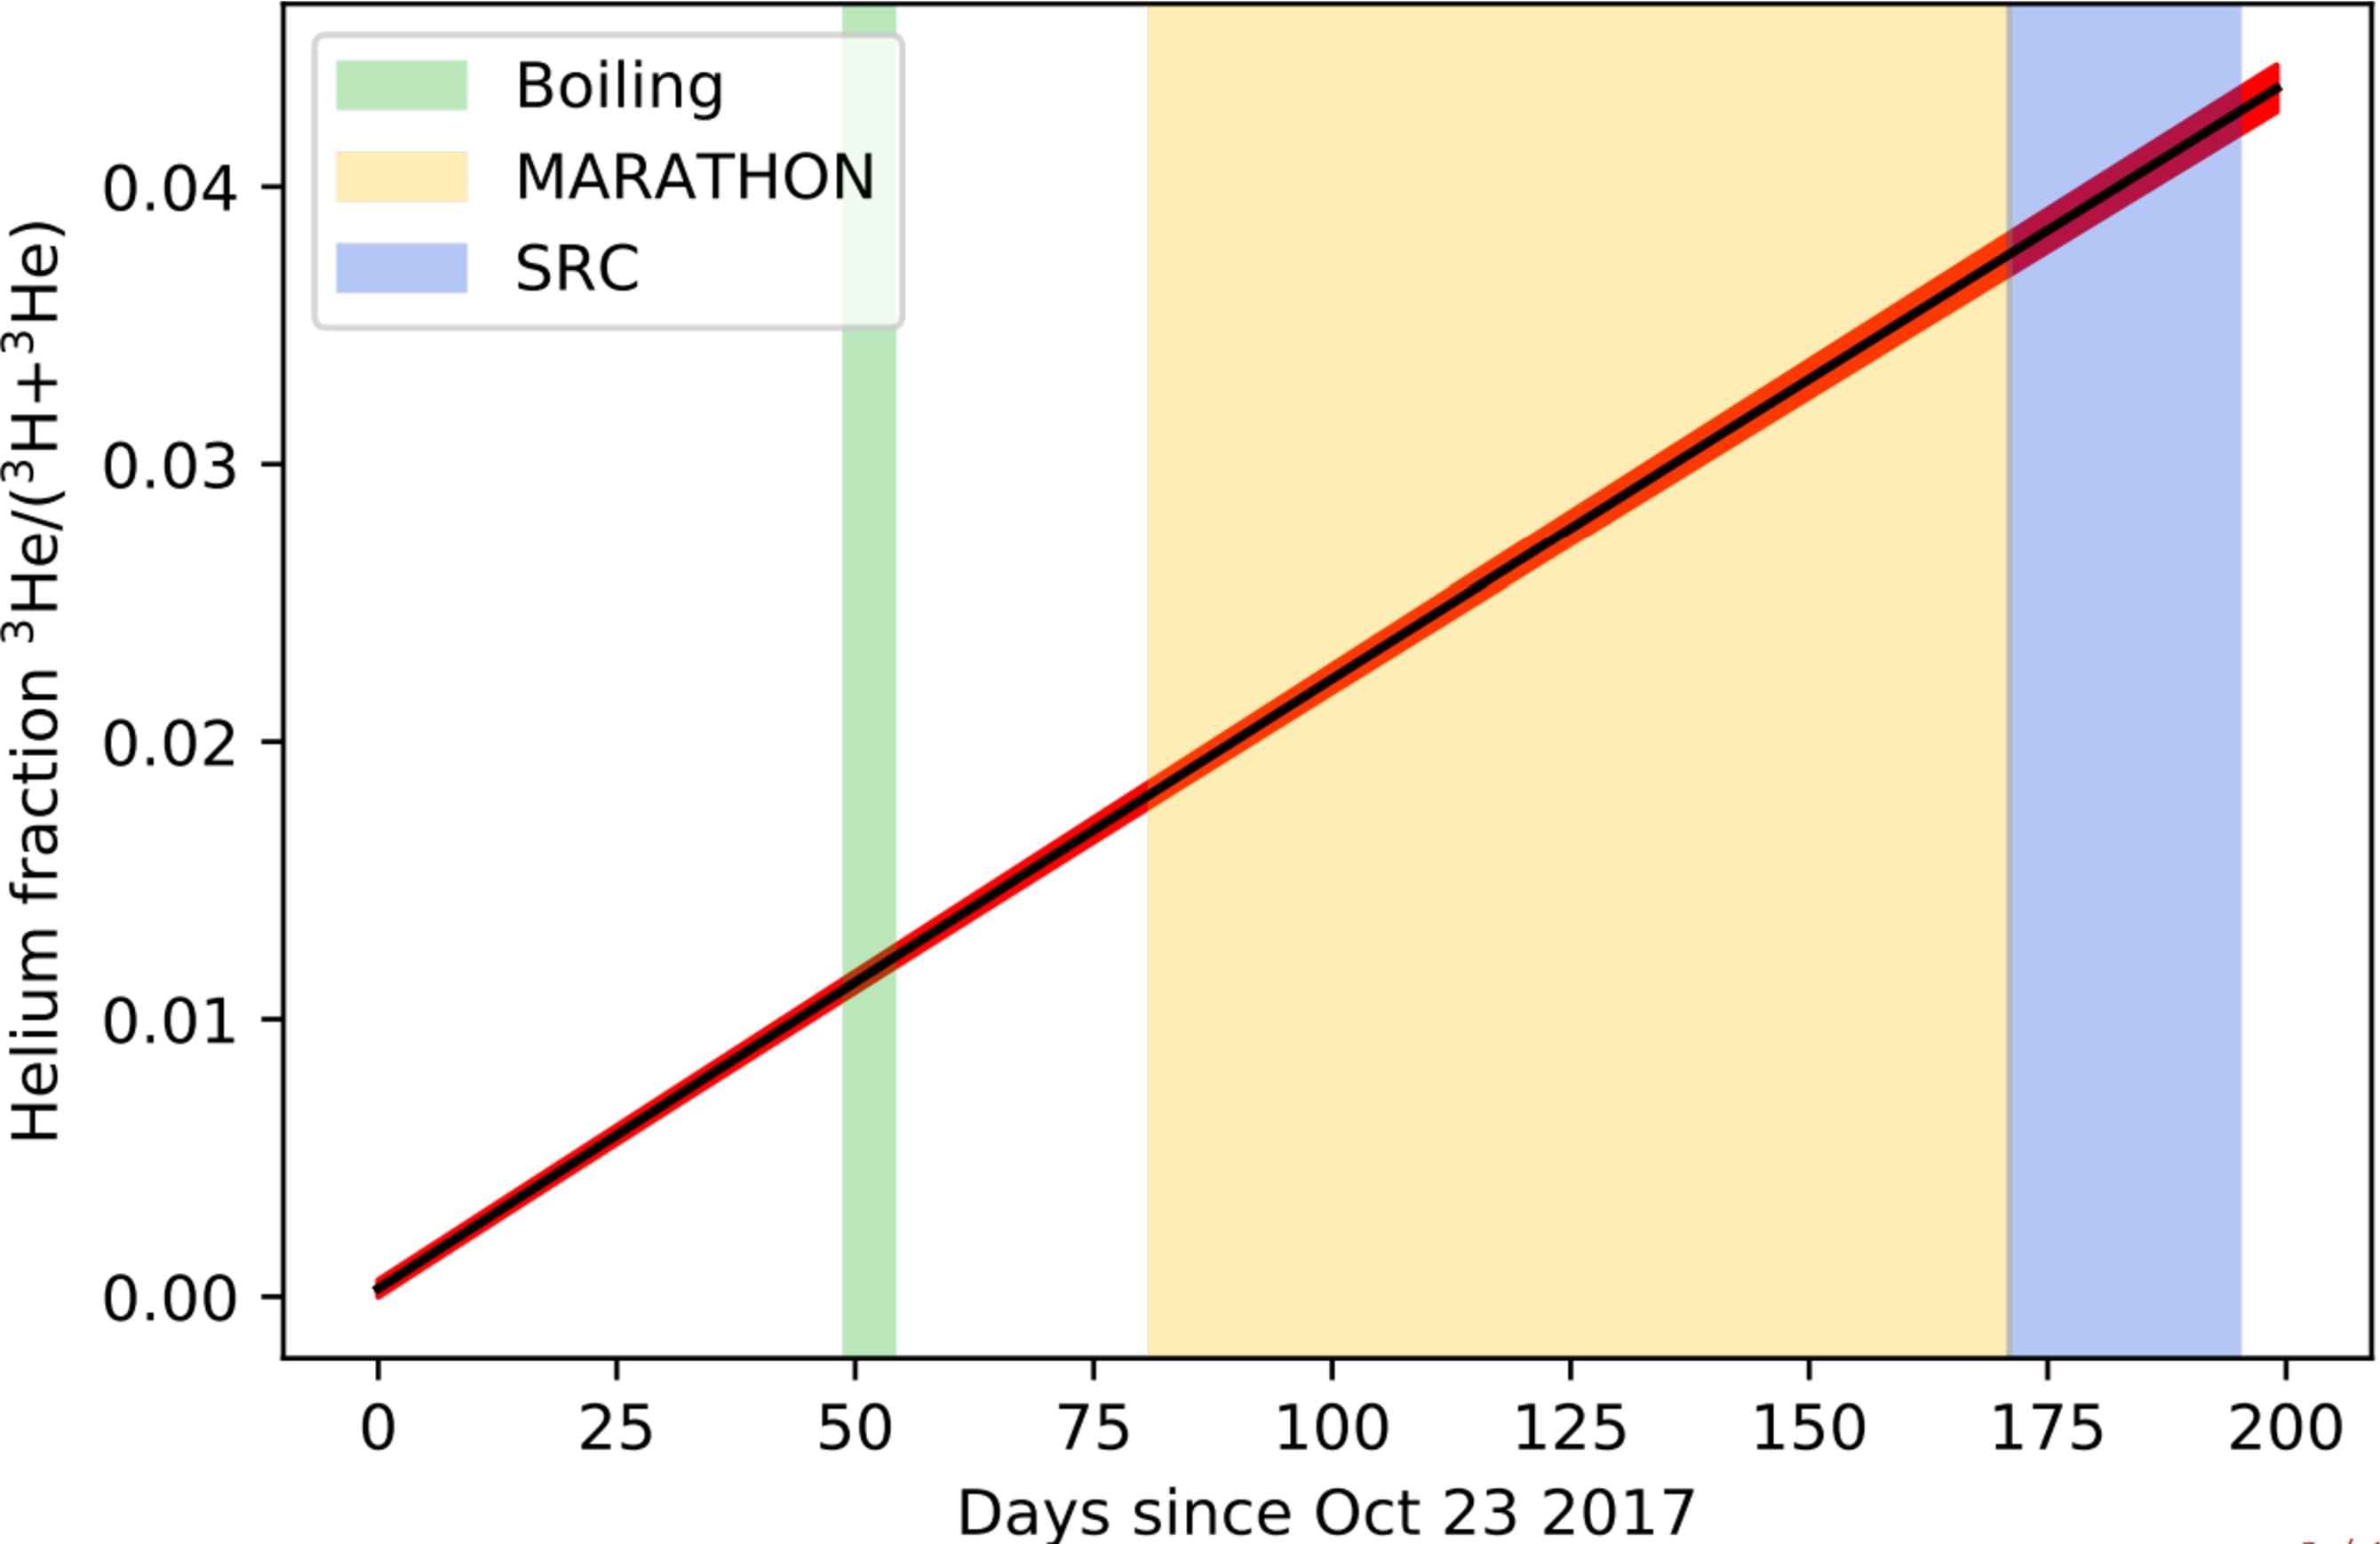
\includegraphics[width=13cm]{cont_Hfrac.pdf}
	\caption{The amount of Helium in the Tritium cell in reference to the total amount of material in the cell as a function of time. Included are bands of time for different sections of the Tritium run group's plan \cite{Beta}.}
	\label{Hfract}
\end{figure}
\begin{equation}
Y = \frac{\sum N_i}{\sum Q_i n_i}, \label{yield} 
\end{equation}
\begin{equation}
Y_{raw} = \frac{\sum (T_i + H_i)}{\sum Q_i (n_{T,i} + n_{H,i})} \label{Yraw}
\end{equation}
\begin{equation}
\langle f_H \rangle \equiv \frac{\sum Q_i f_{H,i}}{\sum Q_i} \label{QwHf}
\end{equation}


The events that scatted from Helium in our tritium cell need to be subtracted from the measured yield to supply an accurate count. The yield from any target is defined as the number of electrons per charge weighted scattering centers. The yield is shown in equation \ref{yield} and defined as the number of counted events($N_i$) per possible scattering changes, or charge($Q_i$) times number of scattering centers ($n_i$). Data is recorded in many runs, so a sum over runs($i$) is required to get the total yield. The subtraction factor is calculated by breaking down the yield from the tritium cell as the addition of the yield from tritium ($Y_T$)= $\Sigma(T_i/Q_in_{i})$ and helium ($Y_H$)= $\Sigma(H_i/Q_in_{i})$ in the tritium cell as shown in equation \ref{Yraw}. The correction for the beta decay is defined in equation \ref{YieldT}. It can be determined by expanding equation \ref{Yraw} out and solving for the tritium yield from the tritium cell. Where $\langle f_H \rangle$ is the charge weighted helium fraction defined in equation \ref{QwHf} \cite{primer}. The helium fraction $f_{H,i}$ is the ratio of helium scattering centers in the tritium cell to total number of scattering centers. 

\begin{equation}
Y_T = Y_{raw}\left(\frac{1}{1-\langle f_H \rangle}\right) - Y_H \left(\frac{\langle f_H \rangle}{1-\langle f_H \rangle}\right) \label{YieldT}
\end{equation}

\section{Luminosity}

\section{Monte Carlo Ratio Method}
Use ECs slides need cite ,explain how to get CS from data/MC

\subsection{Monte Carlo Simulation}
gen - table -weight
\subsection{Monte Carlo Comparison}
acc - comp
\section{DIS Cross Section}

\section{Systematic Error}

